%
% latex-sample.tex
%
% This LaTeX source file provides a template for a typical research paper.
%

%
% Use the standard article template.
%
\documentclass{article}

% The geometry package allows for easy page formatting.
\usepackage{geometry}

\geometry{letterpaper}

% Load up special logo commands.
\usepackage{doc}

% make a reference to Hypertext 
\usepackage{hyperref}

% Package for formatting URLs.
\usepackage{url}
\usepackage{caption}
% Packages and definitions for graphics files.
\usepackage{graphicx}
\usepackage{epstopdf}
\graphicspath{ {C:/Users/ccasstudent/Desktop/Amit_Nayak/GW_MSBA/DNSC_6211/} }
\DeclareGraphicsRule{.tif}{png}{.png}{`convert #1 'dirname #1'/'basename #1 .tif'.png}

%
% Set the title, author, and date.
%
\title{Puzzling Election Results?  \\ \small{DNSC 6211: Programming for Analytics}}
\author{
	Amit Nayak \\
	Soomin Park \\	
	Junfei Zheng \\
	Tianweibao Zheng \\
	Ziqing Zhu \\
}
\date{November 28th, 2016}

%
% The document proper.
%
\begin{document}

% Add the title section.
\maketitle

% Add an abstract.
\abstract{
%Describe your project within 200 words.  One way is answer the following questions regarding your project: (a) what did you do? (b) why did you choose do that? (c) how did you go about doing your project (d) what did you find out?, and finally (e) What did you find out? The content of your abstract and the outline and contents of your report may vary according to the needs of your specific research topic.
%}

Our team collected a variety of data of each state in the United States. The variables we looked at include income levels, GDP, and unemployment rates, among various other variables. We then created one large data set including these variables and tried to run a regression analysis to see if we could develop some sort of formula to predict how the election results would turn out based on our regression equation. We chose to do this to see if such a regression equation could be attained given how surprising the result went in the eyes of many. Additionally, we examined the correlation matrix of variables to eliminate any redundant variables, and used visualization tools such as mapping and shiny to better envision the data that we received for each state. The regression equation we developed is statistically significant in that it does a significantly better job at predicting whether Trump or Hillary wins a state than a model that uses the averages for each variable.


% Add various lists on new pages.
\pagebreak
\tableofcontents


% Start the paper on a new page.
\pagebreak

%
% Body text.
%
\section{Introduction}
\label{introduction}

%You will almost certainly start with an introductory description of the topic that you investigated in your assignment.  Discuss any goals, motivation, or examples of the subject; the key is to provide the reader with any information that is necessary to understand why your topic was worth investigating.  This descriptive section should also allow the reader to understand the subsequent detail sections on the subject. Limit this to 250 words.

The 2016 presidential election will go down as one of the most interesting presidential elections in history. Behind all the chaos that went on with the debates and each candidate's issues and debacles, none of the polls had predicted a Trump victory. Even the remarkable website FiveThirtyEight, which had predicted 101 out of the 102 states (and DC) correctly in the last two presidential elections, failed to predict the outcome of this election cycle correctly. Our group thought it would be of vast interest not just to us, but countless Americans to see if we could determine variable(s) that could help create a regression equation to predict the correct outcomes in each state. Additionally, we want to identify variables that are highly correlated with one another and remove them from our regression model. Finally, we wanted to utilize visualization techniques such as mapping and shiny to help illustrate the data that we received for each individual state for each separate independent variable.


\section{Background}

%Explain your "storyline" and the relevance of the different components. Talk about the nature of the data; why you chose the data you did; how did looking at the data help you decide which dataset(s) to use; and, why? What were the questions that you started with? How did those questions change as you explored the data? Did you give up on some datasets because they were not interesting? Which ones were those? How did you finally end up getting to the question(s) that you finally answered? This entire process is will help me understand how you went about framing the issue(s). Limit this to 250 words.

As with any presidential election, it is always interesting to look at the breakdown of votes among the various demographic groups. This election cycle may have been even more interesting to investigate the breakdown among the various demographics given how divisive the two candidates can be perceived. Given Donald Trump's stance on certain groups of people, such as Mexicans, Muslims, and women to name a few, one would tend to believe that the breakdown among such demographics would be more pronounced than in past election cycles. As a team, we decided to investigate a multitude of variables, which include but are not limited to race, gender, income level, and education levels. If we are able to find a regression equation supporting our numerous variables, it can help us determine which variables strongly support a certain outcome, and which may play a more secondary role.


\section{Method}

%The overall question that you answered
%Any sub-questions
%Any questions that you had but could not respond to satisfactorily (this will not result in a negative grade - but will give me an idea of how you went about your project. Limit this to 250 words.

We first used a web crawler in python to save web page contents into a \textbf{json} file. We then used the keyword extractor from the Monkeylearn library in Python, Twitter API and oAuth for data access and use by using the Tweepy library for visualizing main keywords using the Wordclouds library. Next, we utilized the \textbf{stepAIC()} function from the MASS package to perform stepwise selection. We then proceeded by trying to remove redundant variables via correlation analysis. We were able to do this using R's correlation table, as well as the matplotlib charts to add linear regression lines. We performed Python's matplotlib and seaborn to show pairwise relationships between variables and then drew the detailed correlations table using R to do detailed correlation analysis. We continued on by using the function \textbf{lm} to perform multiple linear regression in R. We then performed python's package sklearn to do cross validation of the models we got and drew comparisons of real and predictive values using matplotlib. We concluded this portion of the regression by using a decision tree to clarify the result. The rpart programs build classification or regression models of a very general structure using a two stage procedure; the resulting models can be represented as binary trees. Rattle provides an interface to R functionality for data mining. The last step was to use a Heatmap from the Plotly Module and Shiny with bubblechart from GoogleCharts to provide us with a visualization of the data.


\section{Organization}

%Describe how you divided up the work in your group. Limit this to 100 words.

Our group divided the work pretty evenly based on what each of our strengths were. Amit was responsible mostly for the documentation, presentations, videos, and analysis. Jeff and Tianweibao played an active role in the data preparation and modeling aspects, especially when it pertained to regression analysis, using R, ggplot, and matplotlib. Ziqing was responsible for the data preparation using python for web scraping and the map programming. Finally, Soomin was responsible for the twitter analysis using python twitter API libraries and oAuth, and R Shiny programming, as well as organization of the presentation.


\subsection{Workflow}

%Provide a diagram of the workflow for your project. The command to include a diagram is shown below. Make sure you \underline{remove the comment} and \underline{change the name of the graphic file} without extension. Also, instead of \textbf{Quick Build} choose \textbf{PDFLaTex} from the dropdown option. Then generate the pdf with \textbf{View PDF}.



\begin{figure}[hb]
  \centering
    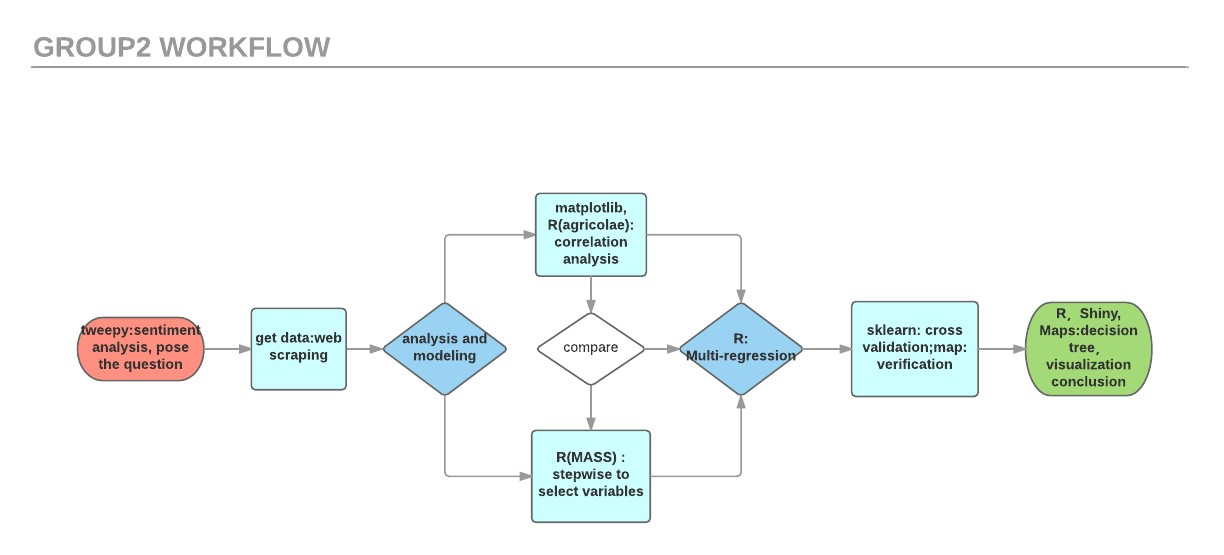
\includegraphics[scale=0.5]{group2workflowv2}
  \caption{The project workflow}

\end{figure}

We first used tweepy to get a sentiment analysis from twitter. We then got our data through web scraping and from downloading the data (when web scrapping wasn't possible). We then did analysis and modeling by comparing the correlation analysis from matplotlib and R's agricolae package, with the stepwise regression we got from R's MASS function. This led to the development of the multivariate regression that we obtained through R. We then proceeded by verifying the model that we got by using sklearm, cross validation, and mapping to make sure that we weren't overfitting our model. We concluded our project by using shiny, a decision tree, and mapping to help us visualize our data and the results that we obtained in order to arrive at our final conclusion of all the work that we did.
%Please explain your workflow diagram in this space. Limit this to 250 words.


\subsection{Project structure}

The main source we used was http://www.bea.gov/regional/downloadzip.cfm. This source enabled us to collect a vast array of data including the state-by-state breakdowns of GDP, income levels, and education levels. We also scraped data from CNN.com and statsamerica.org, while also doing a twitter analysis. These various sources enabled us to get the requisite data for breaking down the various state populations among an assortment of demographics, including race, gender, income levels, and GDP to name a few. This helped enable us to develop a regression equation to help us solve our ultimate goal of attempting to predict the 2016 presidential winner in each of the 50 states and the District of Columbia.
%Describe your data sources. In addition, describe how they are related to each other and to the research question(s). Limit this to 250 words.

\subsection{Figures and Tables}
%
%List your tables and figures and explain why you chose to use them. Explain how these tables and / or figures contribute to your "story." Limit this to 250 words.
%
%\usepackage{placeins}


%
%\begin{minipage}{\linewidth}
%\begin{center}
%\includegraphics[width=.6\linewidth]{example-image}
%\captionof{DataTable}{State-by-State Data}
%\end{center}
%\end{minipage}

\begin{figure}[!h]
 \centering
   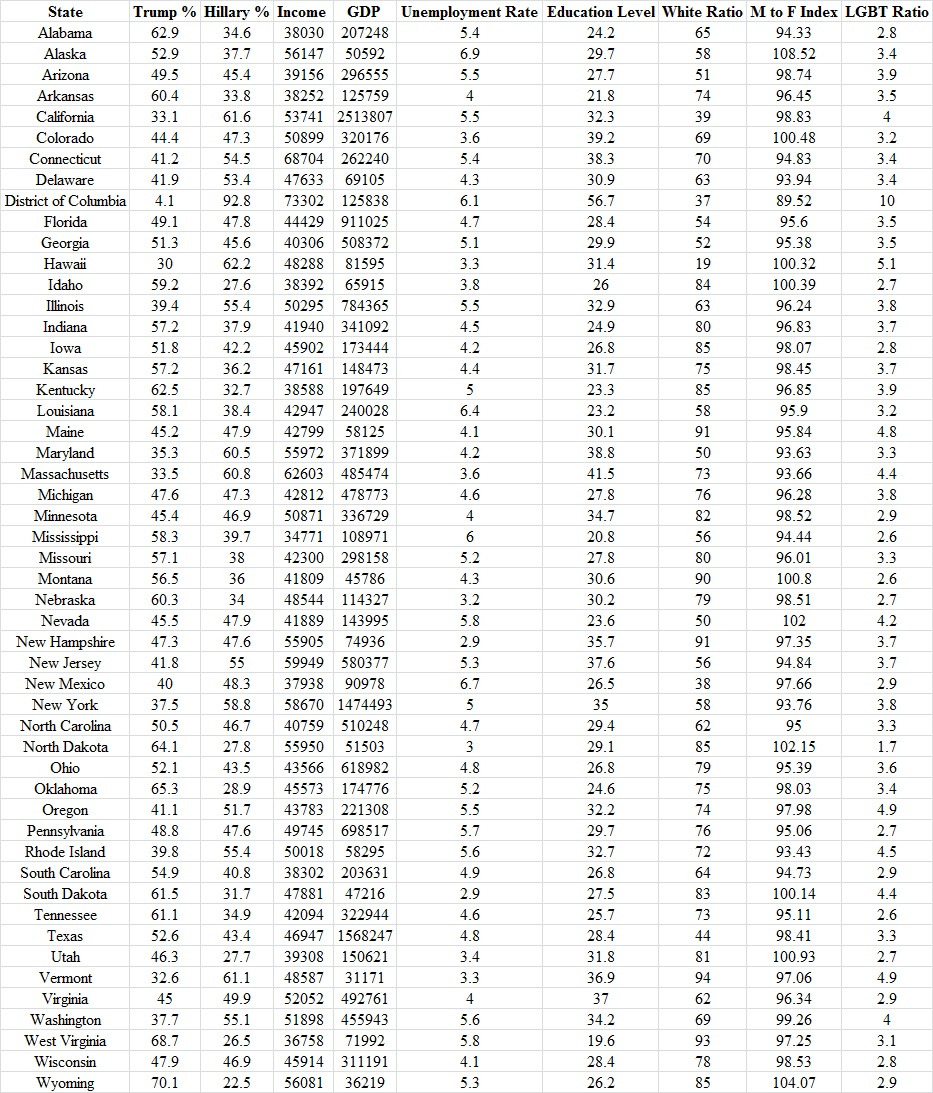
\includegraphics[scale=0.5]{DataTable}
  \caption{State-by-State Data}
\end{figure}  

\begin{figure}[!h]
  \centering
    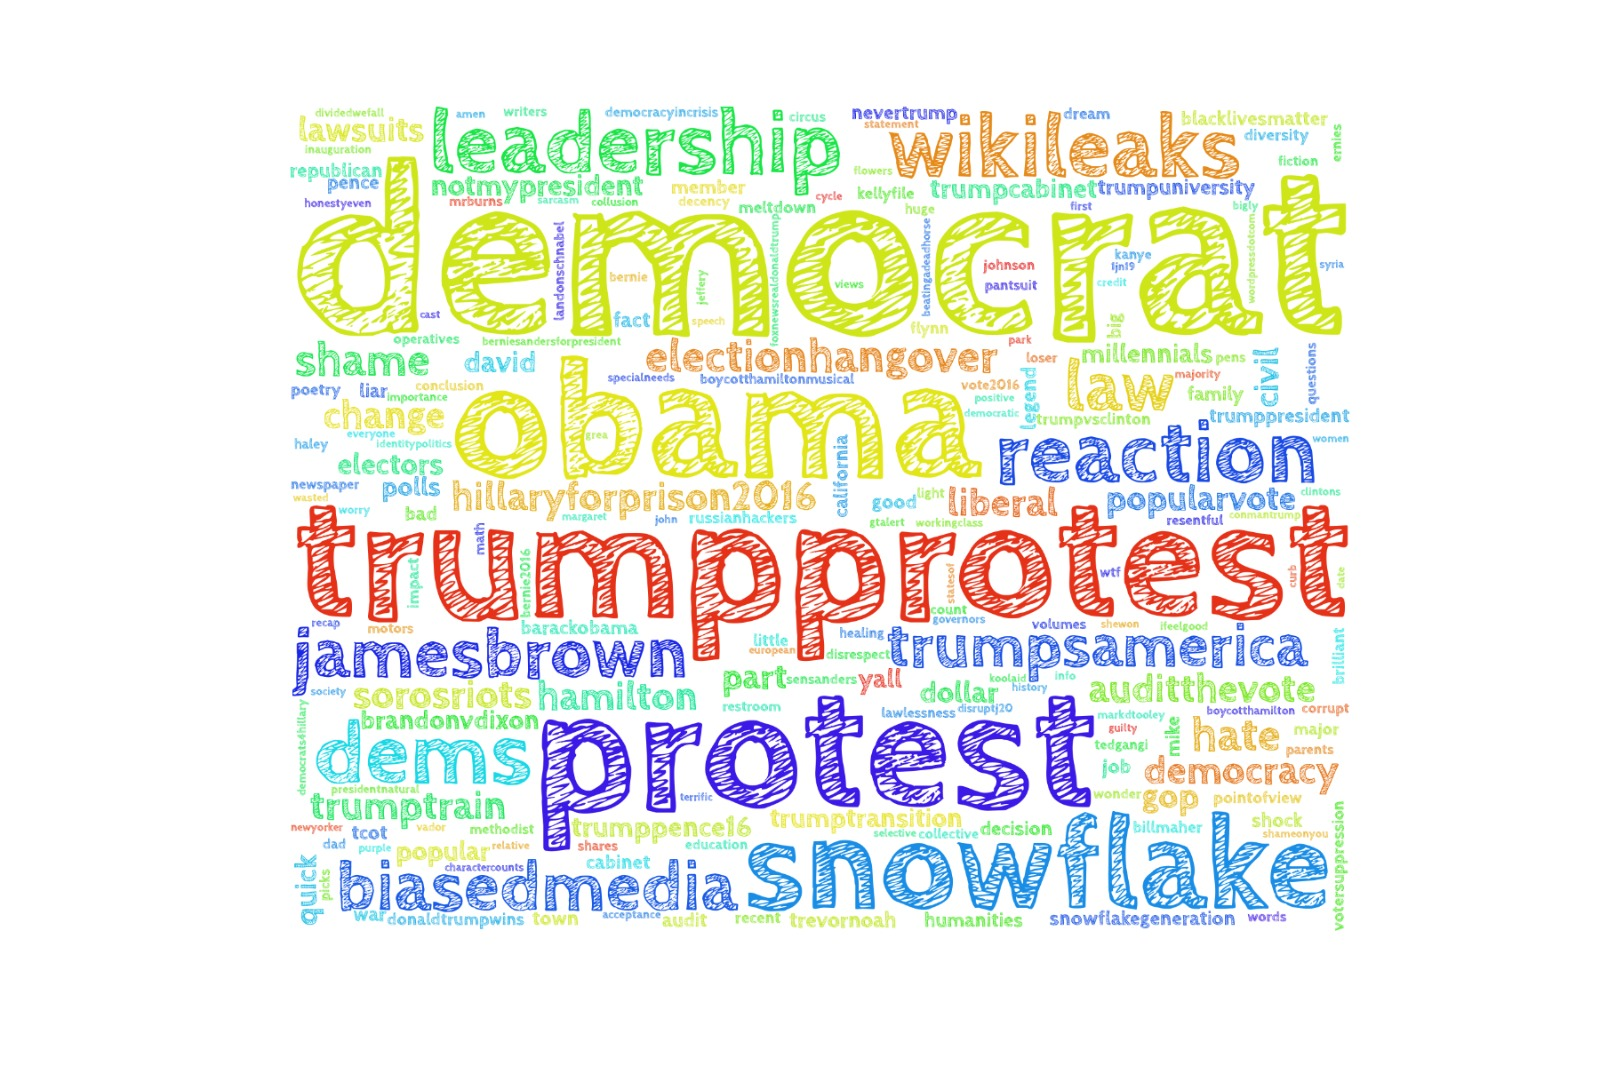
\includegraphics[scale=0.2]{TwitterAnalysis1}
  \caption{1st Twitter WordCloud}
\end{figure}  

\begin{figure}[!h]
  \centering
    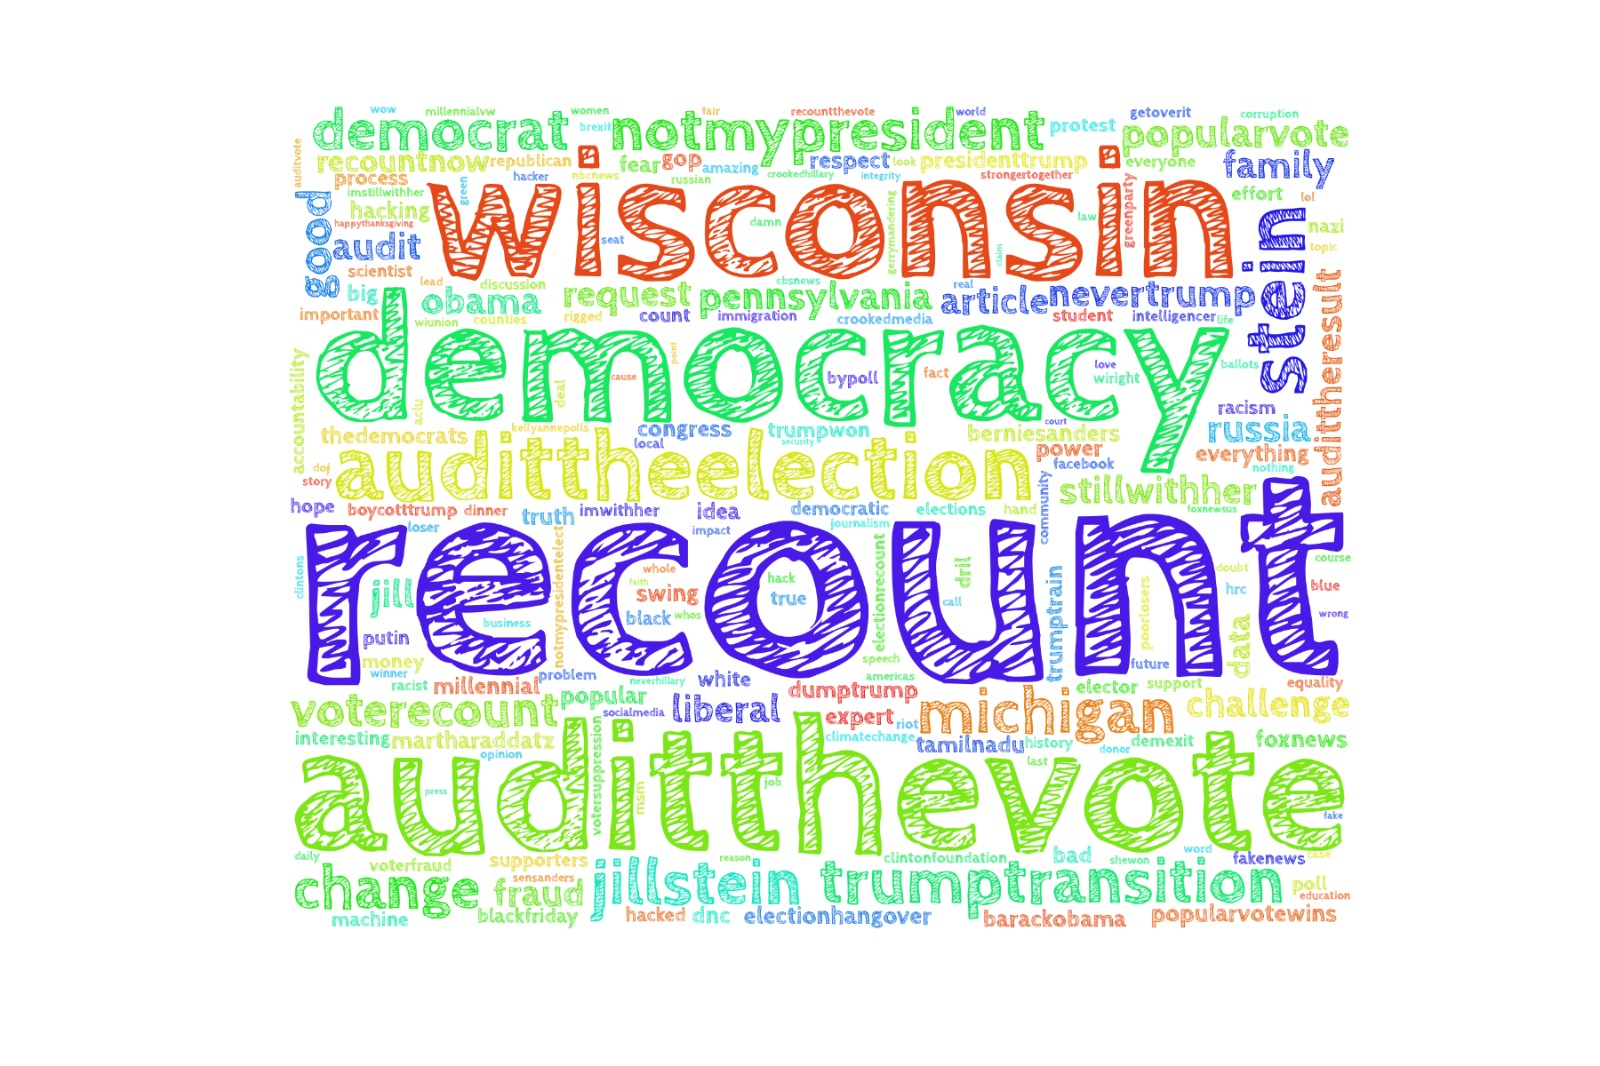
\includegraphics[scale=0.2]{TwitterAnalysis2}
  \caption{2nd Twitter WordCloud}
\end{figure}

\begin{figure}[!h]
  \centering
    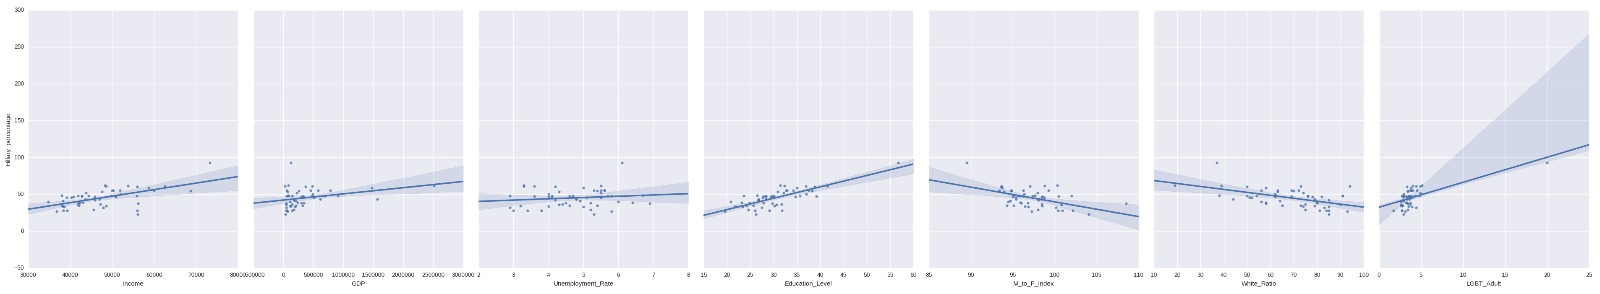
\includegraphics[scale=0.3]{HillarySLR}
  \caption{Single Linear Regression for Clinton}
\end{figure}

\begin{figure}[!h]
  \centering
    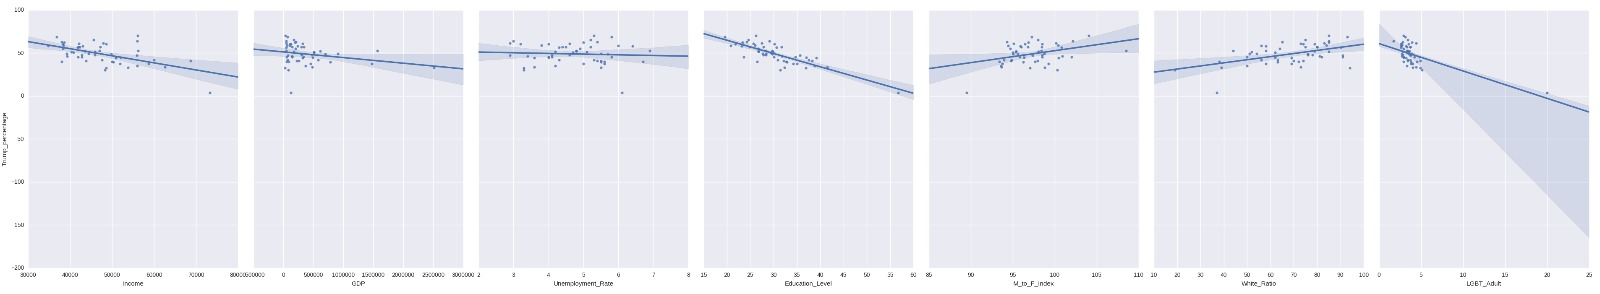
\includegraphics[scale=0.3]{TrumpSLR}
  \caption{Single Linear Regression for Trump}
\end{figure}

\begin{figure}[!htb]
  \centering
    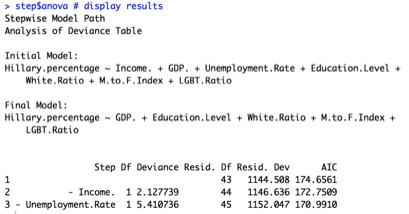
\includegraphics[scale=0.7]{HillaryStepwiseRegression}
  \caption{Stepwise Regression for Clinton}
\end{figure}

\begin{figure}[!htb]
  \centering
    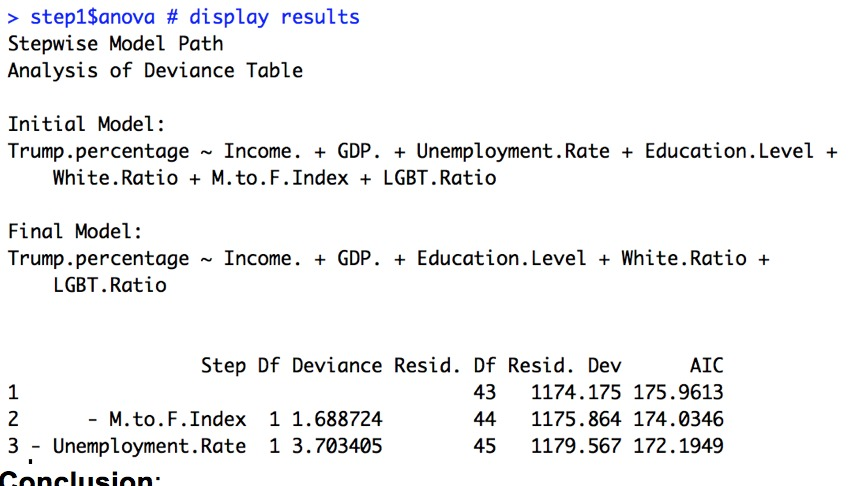
\includegraphics[scale=0.4]{TrumpStepwiseRegression}
  \caption{Stepwise Regression for Trump}
\end{figure}

\begin{figure}[!htb]
  \centering
    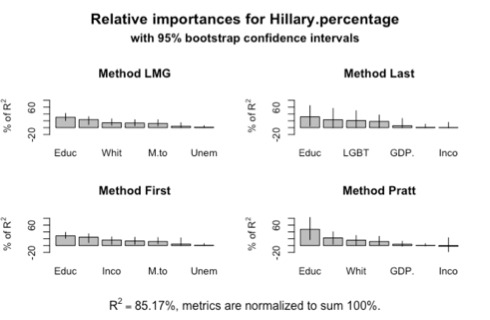
\includegraphics[scale=0.7]{HillaryBootstrap}
  \caption{Variable Impact on Model for Clinton}
\end{figure}

\begin{figure}[!htb]
  \centering
    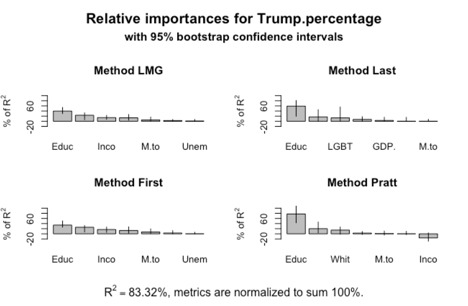
\includegraphics[scale=0.7]{TrumpBootstrap}
  \caption{Variable Impact on Model for Trump}
\end{figure}

\begin{figure}[!htb]
  \centering
    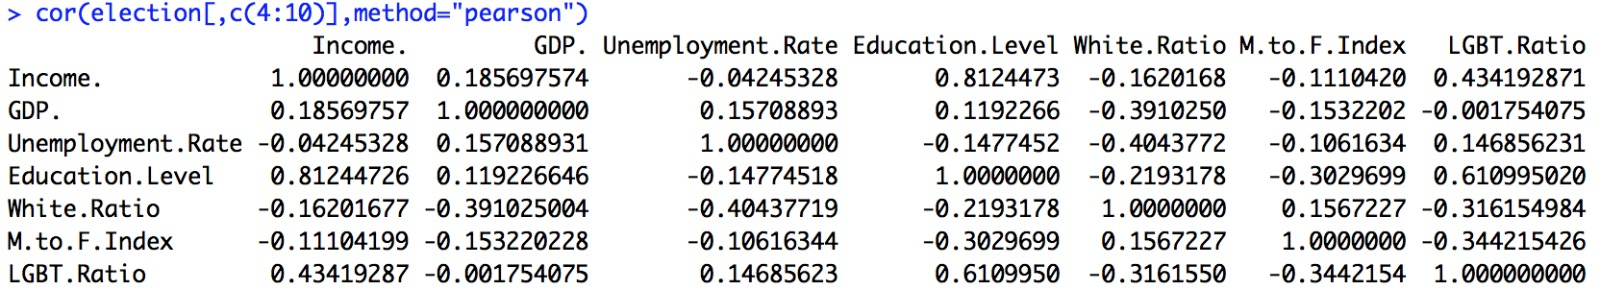
\includegraphics[scale=0.3]{CorrelationMatrix}
  \caption{Correlation matrix of all our independent variables}
\end{figure}

\begin{figure}[!htb]
  \centering
    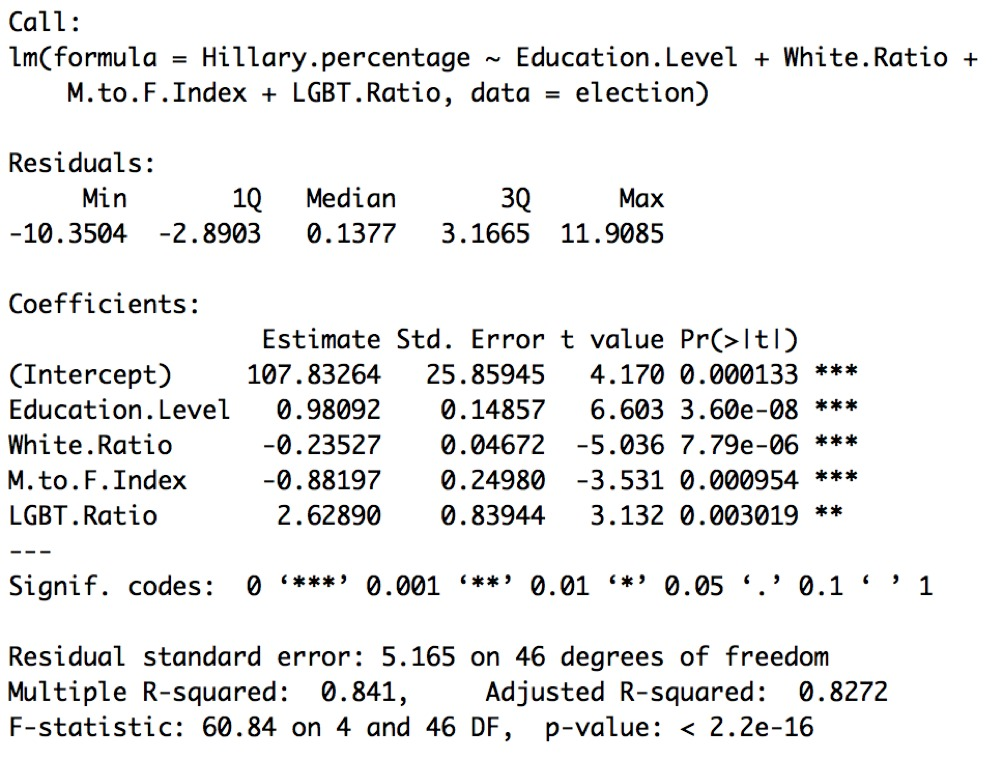
\includegraphics[scale=0.3]{ClintonModel}
  \caption{Final Regression Model for Hillary Clinton}
\end{figure}

\begin{figure}[!htb]
  \centering
    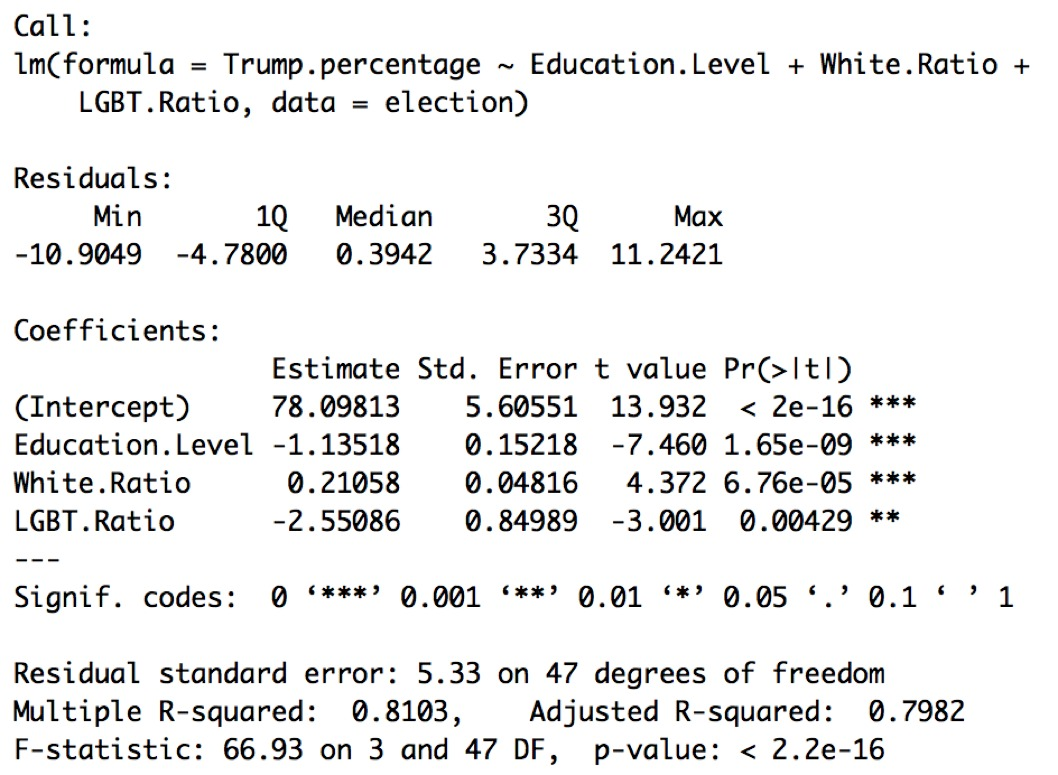
\includegraphics[scale=0.3]{TrumpModel}
  \caption{Final Regression Model for Donald Trump}
\end{figure}

\begin{figure}[!htb]
  \centering
    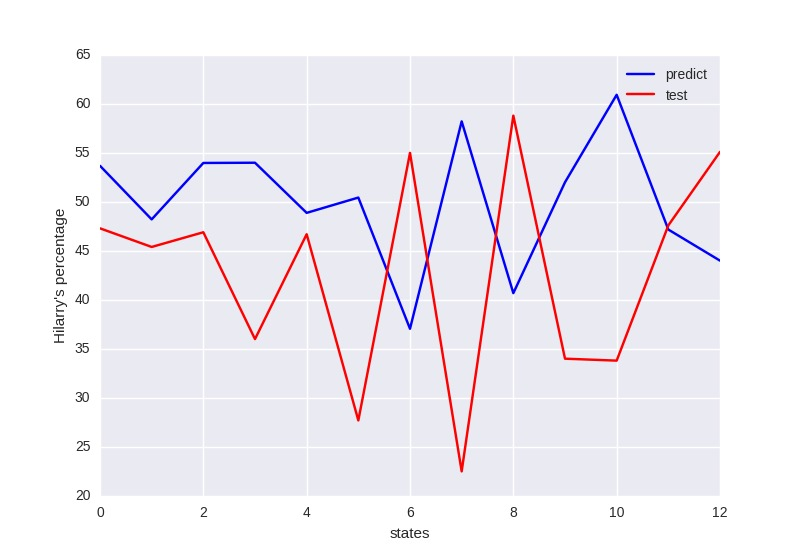
\includegraphics[scale=0.5]{HillaryVerification}
  \caption{Comparison of Clinton Model with the Actual Outcomes}
\end{figure}

\begin{figure}[!htb]
  \centering
    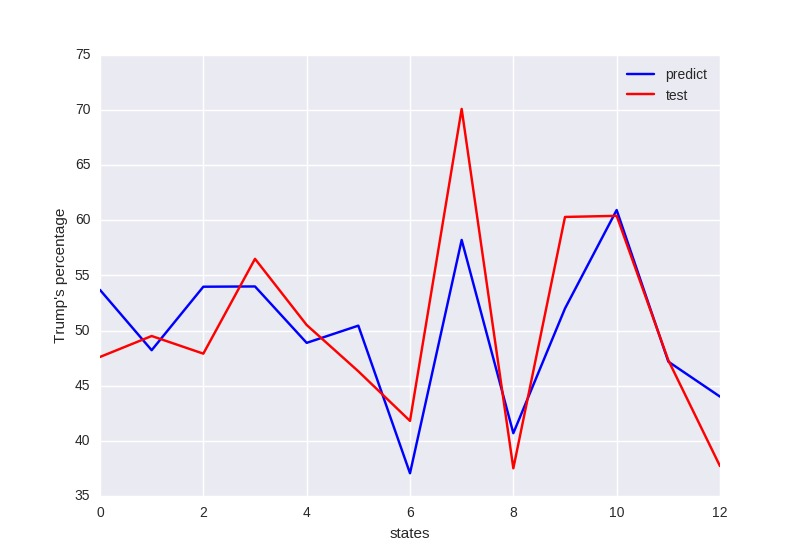
\includegraphics[scale=0.5]{TrumpVerification}
  \caption{Comparison of Trump Model with the Actual Outcomes}
\end{figure}  

\begin{figure}[!htb]
  \centering
    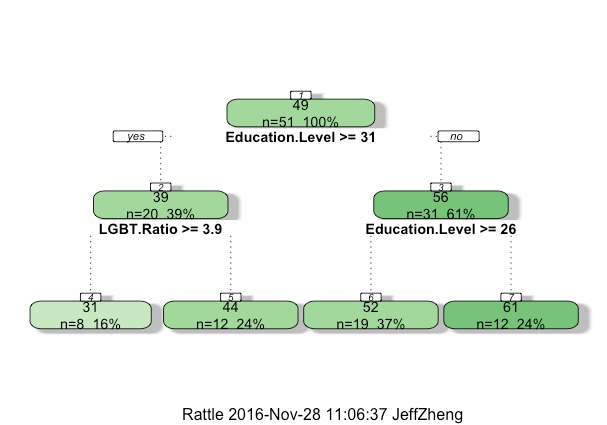
\includegraphics[scale=0.5]{StepwiseClinton}
  \caption{Stepwise Model for Hillary Clinton}
\end{figure}  

\begin{figure}[!htb]
  \centering
    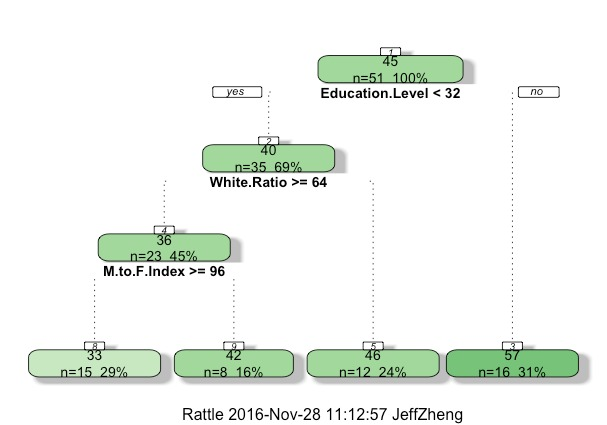
\includegraphics[scale=0.5]{StepwiseTrump}
  \caption{Stepwise Model for Donald Trump}
\end{figure}

\begin{figure}[!htb]
  \centering
    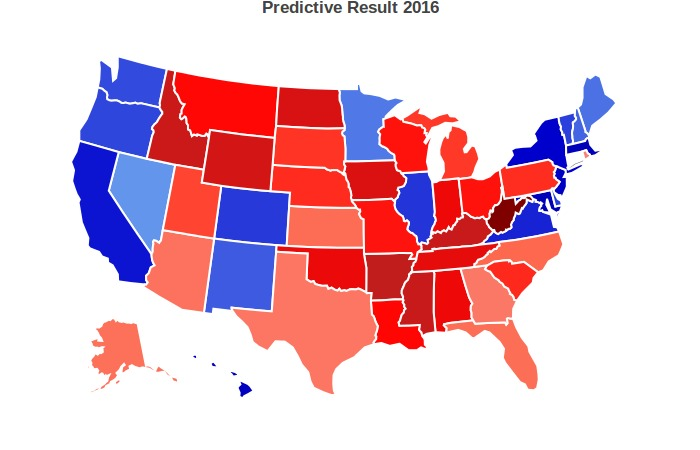
\includegraphics[scale=0.5]{ModelPredictionMap}
  \caption{Map our Model Predicts}
\end{figure}  

\begin{figure}[!htb]
  \centering
    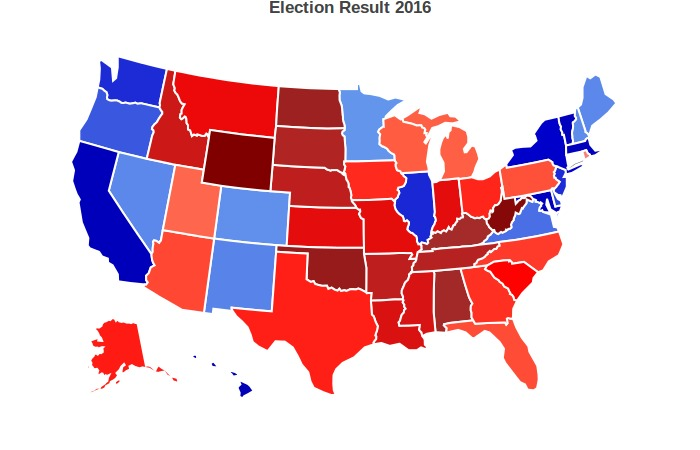
\includegraphics[scale=0.5]{ActualMap}
  \caption{Actual Election Results Map}
\end{figure}  

\clearpage

We started by doing a keyword twitter analysis. More common words are larger in our wordcloud here. There are numerous noteworthy words here, such as protest, audittheelection, and recount. We then scraped all our data into one easy to read data table. Next, we performed simple linear regressions of each variable to find the correlation between each independent variable and the support rate of each candidate. We then developed a stepwise regression model to eliminate variables. For both models we were able to go from 7 variables initially to 5 in our final models here. We then performed four different tests on each model to calculate the contribution that each variable had on our variable. We then got a correlation matrix to help remove even more variables. Variables with a correlation value closer to 1 are highly correlated, so we can remove one of those variables, since they become redundant in our model. We then got a decision tree to break down our data at the cleanest breaks in support rates among all our variables. We then got a map to compare our predictive model with the actual model and you can see that we performed pretty well, getting all 50 states and DC predicted correctly. We finally got our multivariate linear regression. In both models we got our final model down from 7 variables to 3 or 4. Additionally, both models have a high R-squared value of over 80 percent and an extremely statistically significant p-value. We then verified our model to account for the possibility of overfitting. We can see here that our Trump model performed slightly better, but that both models performed pretty well.

\section{Discussion}
%
%This section requires you to discuss your experience. Describe the value of your project. What are two main "selling points" of your project. Limit this to 150 words.
%

The two most significant takeaways from our project were the multiple regression analysis and the visualization that we were able to obtain. The multiple regression analysis enabled us to figure out which variable(s) played the most significant role in our regression model. We were able to determine that two most significant factors in our model were the education level and the ratio of white people. Higher ratios of white people and lower education levels were associated with a higher support rate for Trump and vice versa for Clinton. The visualization methods we utilized, mapping and shiny, also helped created a very easy-to-read interpretation of the election results along each of the numerous variables that we utilized. For the shiny, we used the Google charts library and were able to provide a scatter plot chart for each of the independent variables with their relationship with the dependent variable (support rate for each candidate). Additionally, we were able to designate each state into one of the six basic regions in the US and adjust the size of each dot based on how many electoral votes that state was worth.

%Multiple regression analysis
%	education level and ratio of white people - most important
%	relationship with support rate
%Visualization - using mapping and shiny (google charts library)


\subsection{Learnings}
%
%Discuss some of your "better moments" in this projects - the ones you enjoyed. Also describe. what you learned in this project. Limit to 150 words
%

There were a few things that we learned in addition to our main takeaways from this project. One precious lesson we learned from the project is how to build the model. Selecting a certain number of variables from thousands of possibilities is not easy. First, we had to take a glance over all the variables and then guess the possible driving factors that will be added into our initial formula. Then, identifying and creating the model required strict logic to execute. Finally, we needed to evaluate the final model to make sure that the result we obtained was a reliable one. We also learned to use plotly when created our map. We needed this to combine the two kinds of maps into our final map. We then divided the maps into two submaps and represented each with a different color.

%We were able to use shiny to visualize the effects each individual variable had on the support rate for each Clinton and Trump. We were also able to break down each state into one of the six main geographical regions in the United States, thus making it easier to find the correlations between variables and each region.

\subsection{Challenges}
%
%Discuss some of your "difficult moments" in completing this project. You may want to write about things you wanted to do but could not complete and why. Limit to 150 words.
%
We encountered a wide variety of challenges throughout the duration of this assignment. One basic issue was choosing only a certain amount of variables to examine. As is commonly known, there are countless different variables that can be examined when it comes to presidential elections. After choosing the variables we wanted to investigate, we then had to web scrape the data, where we came across a few more obstacles. Some sources didn't allow us to scrape their data, while a few others gave us unusable HTML code, instead of data. Utilizing multiple variables also gave us additional challenges when running our shiny. We were only able to investigate each independent variable's relationship independently with their correlation on the dependent variable. We were unable to find a way of running a multivariate shiny program. Finally, when running our twitter analysis, we came across a variety of time-sensitive issues when trying to gather the twitter analysis. 

%Some of the challenges our group encountered include 
%Which variables to select; there are countless amount of variables we could choose to examine
%Webscraping, some web sites don't allow you to web scrape for data
%If you scrape from web site, you will only get HTML code and no actual data
%Too many words to test for in the sentimental analysis; we cannot get more than 3000 tweets in 15 minutes (there is a time limit)
%Can't get the old tweets, could only get tweets from a week before and from the current date
%
%\section{Bullets and numbered lists (FYI, delete in your report)}
%
%This is up to you. If you want to add another section. This section explains how to make lists. In you final report you should delete this part. 
%
%\subsection{Bulleted and Numbered Lists}
%
%\LaTeX\ is very good at providing clean lists.  Examples are shown below.
%
%\begin{itemize}
%\item Bulleted items come out properly indented and spaced, every time.
%
%\begin{itemize}
%\item Sub-bullets are a virtual no-brainer: just nest another \verb!itemize! block.
%\item Note how the bullet character automatically changes too.
%\end{itemize}
%
%\item Just keep on adding \verb!\item!s\ldots
%
%\item \ldots until you're done.
%\end{itemize}
%
%Numbered lists are almost identical, except that you specify \verb!enumerate! instead of \verb!itemize!.  List items are specified in exactly the same way (thus making it easy to change list types).
%
%\begin{enumerate}
%\item A list item
%\item Another list item
%\item A list item with multiple nested lists
%
%\begin{itemize}
%\item Nested lists can be of mixed types.
%\item That's a lot of power and flexibility for the price of learning a handful of directives.
%
%\begin{enumerate}
%\item Like nested bullet lists, nested numbered lists also ``intelligently'' change their numbering schemes.
%\item Meanwhile, all \emph{you} have to write is \verb!\item!.  \LaTeX\ does the rest.
%\end{enumerate}
%\end{itemize}
%
%\item Back to your regularly scheduled list item
%
%\end{enumerate}
%
%BTW, this is a great site to generate tables in Latex and learn how to do it in Latex -- \url{http://www.tablesgenerator.com/}
%
%
\section{Conclusion}
%
%Wrap up your paper with an executive summary of the paper itself, reiterating its subject and its major points. Limit this to 150 words.

We were able to obtain a regression model of all the relevant independent variables that we examined. Additionally, we were able to see which variables had the most significant impacts on the election and what they meant in terms of the support rate for each of the candidates. The two most significant variables that we found were education level and the ratio of white people in each state. We were able to determine that higher education levels and a lower ratio of white people was correlated with a higher support rate for Clinton and a lower support rate for Trump and the exact opposite also held true. We were further able to visualize these trends using the visualization tools of mapping and shiny. Here we were able to better examine these trends of each independent variable and see their correlation with the support rate of each candidate. 

\section{References}
Bea.gov 
\newline CNN.com 
\newline statsamerica.org 
\newline Twitter.com 

\end{document}

